\documentclass[12pt]{article}
\usepackage{amsmath,amssymb,enumerate,enumitem}%la base
\usepackage{fancyhdr}%pour custom les en-têtes et pieds de page
\usepackage[table]{xcolor}%pour les couleurs
\usepackage[a4paper,lmargin=1cm,rmargin=1cm,tmargin=1cm,bmargin=2cm]{geometry}
\usepackage[T1]{fontenc}
\usepackage{hyperref}%hyperliens
\usepackage{graphicx}%images
\usepackage[most]{tcolorbox}%pour les encadrés
\usepackage{import} % pour importer
\usepackage{listings}%pour afficher du code R
\usepackage[pages=some]{background} % pour la page de garde
\usepackage{subcaption}

% --- Couleur violet thème ---
\definecolor{ensae}{RGB}{71, 1, 125}

\hypersetup{
    colorlinks = true,
    linkcolor = ensae!70!white,
    filecolor = ensae,      
    urlcolor = ensae,
    pdfpagemode = FullScreen,
    pdftitle = Linear Time Series Assignment,
    pdfauthor = Alban Géron
}

\pagestyle{fancy}
\lhead{} \rhead{} \lfoot{} \rfoot{}
\renewcommand{\headrulewidth}{0pt}\renewcommand{\footrulewidth}{0pt}

% --- Configuration R ---
\definecolor{codegreen}{rgb}{0,0.6,0}
\definecolor{codegray}{rgb}{0.5,0.5,0.5}
\definecolor{customyellow}{rgb}{1,1,0}
\lstset{
    language=R,                         % R par défaut
    commentstyle=\color{codegreen},
    keywordstyle=\color{blue},
    numberstyle=\tiny\color{codegray},
    stringstyle=\color{magenta},
    basicstyle=\ttfamily,
    breakatwhitespace=false,         
    breaklines=true,                 
    captionpos=b,                    
    keepspaces=true,                 
    numbers=left,                    
    numbersep=3pt,                  
    showspaces=false,                
    showstringspaces=false,
    showtabs=false,                  
    tabsize=2,
    literate=%
        {é}{{\'e}}1 {è}{{\`e}}1 {à}{{\`a}}1 {ù}{{\`u}}1 {â}{{\^a}}1 {ê}{{\^e}}1 {î}{{\^i}}1 {ô}{{\^o}}1 {û}{{\^u}}1
        {É}{{\'E}}1 {È}{{\`E}}1 {À}{{\`A}}1 {Ù}{{\`U}}1 {Â}{{\^A}}1 {Ê}{{\^E}}1 {Î}{{\^I}}1 {Ô}{{\^O}}1 {Û}{{\^U}}1
        {ç}{{\c{c}}}1 {Ç}{{\c{C}}}1
}
\newcommand\rcode[1]{{\lstinline[language=R]!#1!}}

% --- Titres ---
\usepackage{titlesec}
\renewcommand{\thesection}{\Roman{section}} % Titres sections en chiffres romains
\titleformat{\section}{\normalfont\sffamily\bfseries\Large}{\thesection}{1em}{}
\titleformat{\subsection}{\normalfont\sffamily\bfseries\large}{\thesubsection}{1em}{}
\titleformat{\subsubsection}{\normalfont\sffamily\bfseries}{\thesubsubsection}{1em}{}
\setlist[enumerate]{
    font = \color{ensae!70!white}\sffamily,
    leftmargin = *,
    resume
}

% --- Macros ---
\DeclareMathOperator*{\argmin}{arg\,min}
\DeclareMathOperator*{\Var}{Var}
\newcommand{\ARMA}{\textsf{ARMA}}
\newcommand{\ARIMA}{\textsf{ARIMA}}
\newcommand{\AIC}{\textsf{AIC}}
\newcommand{\BIC}{\textsf{BIC}}
\newcommand{\WN}{\textsf{WN}}
\newcommand{\iidsim}{\overset{\text{i.i.d.}}{\sim}}



\begin{document}
    \backgroundsetup{
        scale = 1,
        angle = 0,
        opacity = 1,
        contents = {
            
\includegraphics[width = \paperwidth, height = \paperheight, keepaspectratio]{bgcover.pdf}
        }
    }
   \BgThispage
    \newgeometry{
        lmargin=1cm,
        rmargin=7cm,
        tmargin=4cm,
        bmargin=4cm
    }
    \thispagestyle{empty} % pas de numérotation pour cette page
    \begin{center}
        
\includegraphics[width=0.8\textwidth]{ensae IP paris.png}

        \vskip4cm

        \Large\bfseries
        \begin{tcolorbox}[
            enhanced, sharp corners,
            colback = ensae!5!white,
            colframe = ensae!60!white,
            boxrule = 0.5pt,
            drop fuzzy shadow = gray
        ]
            \centering {\huge\sffamily ARIMA modelling of a time series}

            \vskip0.3cm

            \emph{\Large Linear Time Series Assignment}
        \end{tcolorbox}

        \vskip4cm

        Alban \textsc{Géron} and Théo \textsc{Lartigau}

        \vskip0.5cm

        Academic year: 2024-2025
    \end{center}

    \newpage
    \restoregeometry

    \section{The data}

    \begin{enumerate}
        \item The chosen series is the \emph{seasonally and working-day adjusted Industrial Production Index (IPI) for the manufacture of beverages}\footnote{\url{https://www.insee.fr/fr/statistiques/serie/010767669}}. It tracks the monthly physical output of France’s drinks industry (breweries, wineries, distillers, soft‑drink plants and bottled‑water facilities), adjusted for calendar and seasonal fluctuations. The index is expressed on a base‑$100$ scale with 2021 as the reference year, that is, a value of $110$ means the beverage industry produced $10 \%$ more than its 2021 average in that month.

        To isolate the monthly industrial production data, rows should be filtered to retain only those whose first column matches the \texttt{YYYY-MM} format. The second column, containing the index values, should then be extracted and converted to numeric form. Because the data appears in reverse chronological order, the values should be reversed to restore proper temporal sequencing.

        Although the base‑$100$ scaling tends to keep the variance relatively stable, a logarithmic transformation may still be considered if volatility appears to increase with the level of the index.

        \item As a first step we have checked the stationarity of the initial series, which we will label $(Y_t)$ in the following. Table \ref{tab:stationarity_tests} summarizes the results of the Augmented Dickey-Fuller (ADF), Phillips-Perron (PP) and Kwiatkowski-Phillips-Schmidt-Shin (KPSS) tests. The results of the three stationarity tests on the initial series are somewhat contradictory. Both the ADF and PP tests reject the null hypothesis of a unit root at the $5 \%$ level, suggesting that the series is stationary. However, the KPSS test rejects the null hypothesis of level stationarity, indicating that the series is not stationary. This discrepancy calls into question the stationarity of $(Y_t)$. To determine the integration order of $(Y_t)$, we test the stationarity of the first-order differenced series $(\nabla Y_t)$. Plotting the series $(\nabla Y_t)$ shows that it seems stationary, see Figure \ref{fig:plot_series_diff}. We then applied the same tests to the first-differenced series to determine its integration order, the results of which can be found in Table \ref{tab:stationarity_tests_diff}. Once again, ADF and PP tests reject the null hypothesis of a unit root, however now KPSS accepts the null hypothesis of stationarity at the $5 \%$ level. We conclude that $(Y_t) \sim I(1)$.
        %
        \begin{figure}[ht]
            \centering
            \begin{minipage}{0.48\linewidth}
                \centering
                \begin{tabular}{l|ccc}
                    \textbf{Test} & \textbf{Test Statistic} & \textbf{p-value} & \textbf{Decision} \\
                    \hline
                    ADF  & -4.7236 & < 0.01 & Stationary \\
                    PP   & -148.75 & < 0.01 & Stationary \\
                    KPSS & 5.8263  & < 0.01 & Not Stationary
                \end{tabular}
                \captionof{table}{Stationarity test results on $(Y_t)$}
                \label{tab:stationarity_tests}
            \end{minipage}
            \hfill
            \begin{minipage}{0.48\linewidth}
                \centering
                \begin{tabular}{l|ccc}
                    \textbf{Test} & \textbf{Test Statistic} & \textbf{p-value} & \textbf{Decision} \\
                    \hline
                    ADF  & -10.088  & < 0.01 & Stationary \\
                    PP   & -438.51  & < 0.01 & Stationary \\
                    KPSS & 0.0465   & > 0.1  & Stationary
                \end{tabular}
                \captionof{table}{Stationarity test results on $(\nabla Y_t)$}
                \label{tab:stationarity_tests_diff}
            \end{minipage}
        \end{figure}

        \begin{figure}[h]
            \centering
            \begin{subfigure}[b]{0.49\linewidth}
                \centering
                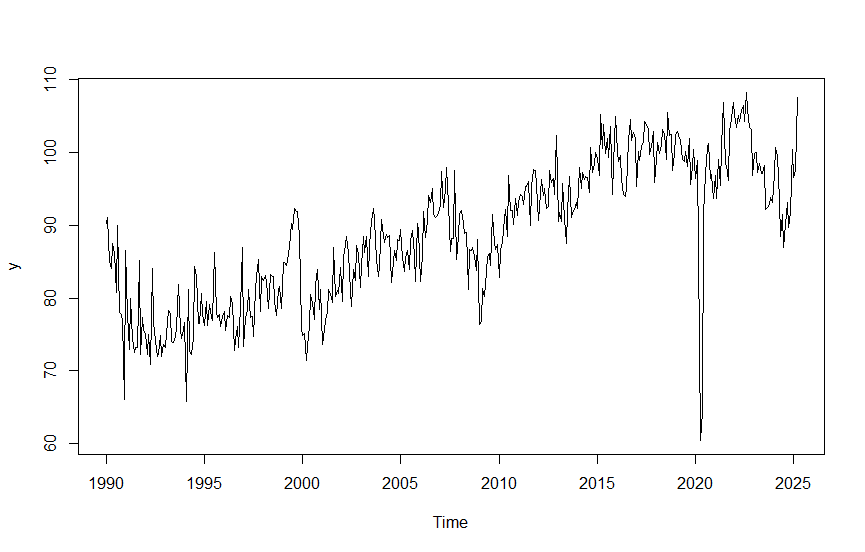
\includegraphics[width=\linewidth]{plot series.png}
                \caption{Initial series}
                \label{fig:plot_series}
            \end{subfigure}
            \hfill
            \begin{subfigure}[b]{0.49\linewidth}
                \centering
                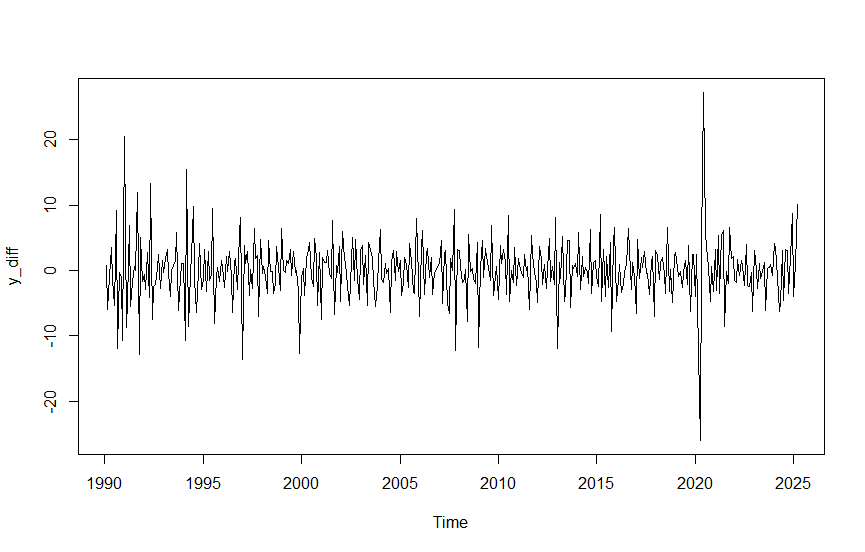
\includegraphics[width=\linewidth]{plot y_diff.png}
                \caption{First-order differenced series}
                \label{fig:plot_series_diff}
            \end{subfigure}
            \caption{Plots of the series $(Y_t)$ and $(\nabla Y_t)$}
            \label{fig:plots_two_series}
        \end{figure}

        \item The plots of the series $(Y_t)$ and $(\nabla Y_t)$ can be found on Figure \ref{fig:plots_two_series}.
    \end{enumerate}

    \section{ARMA models}

    \begin{enumerate}
        \item We seek to fit an $\ARMA(p, q)$ model on the differenced series. The autocorrelograms for the autocorrelation function (ACF) and the partial autocorrelation function (PACF) of the differenced series can be found on Figure \ref{fig:autocorrelograms}.
        %
        \begin{figure}[h]
            \centering
            \begin{subfigure}[b]{0.49\linewidth}
                \centering
                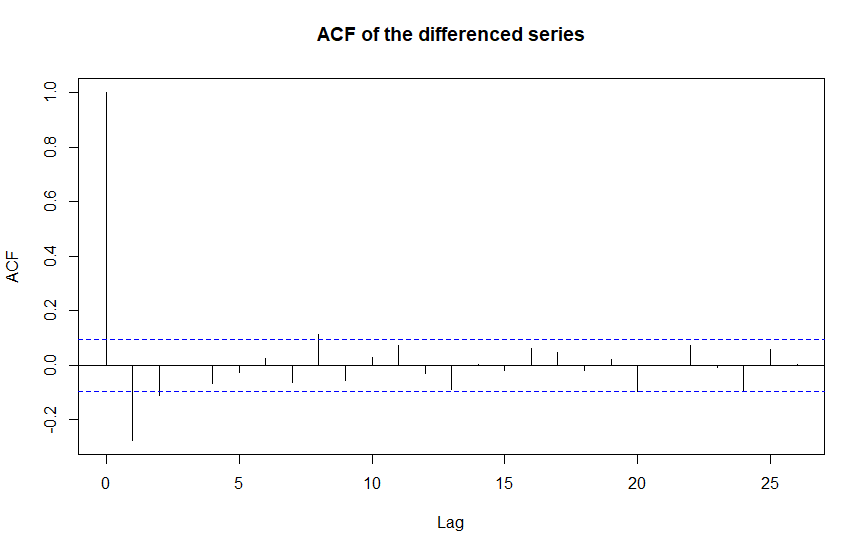
\includegraphics[width=\linewidth]{ACF ydiff.png}
                \caption{ACF of $(\nabla Y_t)$}
                \label{fig:acf_ydiff}
            \end{subfigure}
            \hfill
            \begin{subfigure}[b]{0.49\linewidth}
                \centering
                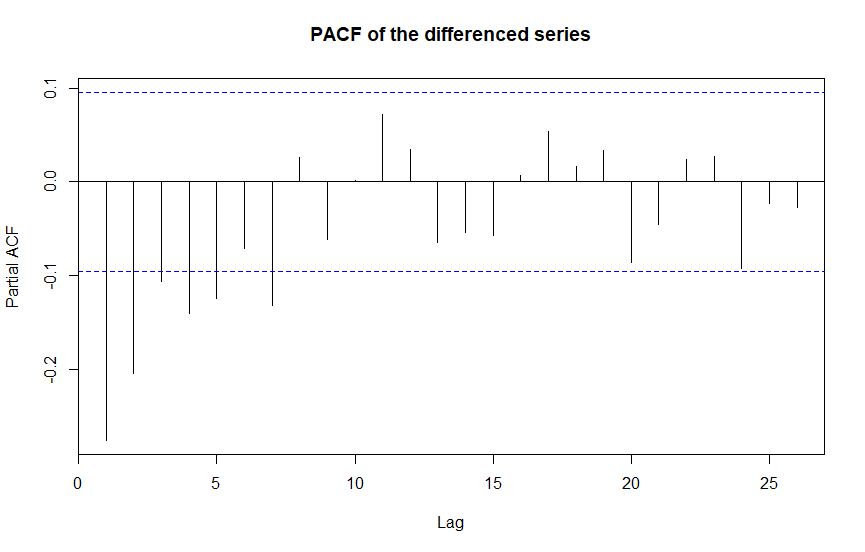
\includegraphics[width=\linewidth]{PACF ydiff.png}
                \caption{PACF of $(\nabla Y_t)$}
                \label{fig:pacf_ydiff}
            \end{subfigure}
            \caption{Autocorrelograms of the differenced series}
            \label{fig:autocorrelograms}
        \end{figure}

        Figure \ref{fig:acf_ydiff} shows that the autocorrelations become non-significant beyond lag 13, while Figure \ref{fig:pacf_ydiff} shows that the partial autocorrelations become non-significant beyond lag 7. Therefore, we seek for the best $\ARMA(p, q)$ for $p = 0, 1, \dots, 7$ and $q = 0, 1, \dots, 13$. To compare those models we find $(p_{\AIC}, q_{\AIC}) \in \argmin_{(p, q)} \AIC(p, q)$ and $(p_{\BIC}, q_{\BIC}) \in \argmin_{(p, q)} \BIC(p, q)$. The results of those two minimization programs, which can be found in Table \ref{tab:aic_bic_results}, suggest that the two best candidates are $(p, q) = (4, 4)$ (minimizing the $\AIC$ criterion) and $(p, q) = (1, 1)$ (minimizing $\BIC$). We note that, in both models, there is only one coefficient that is not statistically significant (see Table \ref{tab:arma44_coeffs} and Table \ref{tab:arma11_coeffs}). Because we foster simplest models to prevent overfitting, we choose to fit the $\ARMA(1, 1)$ model on the series $(\nabla Y_t)$ in the following.
        %
        \begin{table}[ht]
            \centering
            \begin{tabular}{l|ccc}
                \textbf{Criterion} & \textbf{Best $\ARMA(p, q)$ Model} & \textbf{$\AIC(p, q)$} & \textbf{$\BIC(p, q)$} \\
                \hline
                $\AIC$  & $(p, q) = (4, 4)$ & 2417.044 & 2457.494 \\
                $\BIC$  & $(p, q) = (1, 1)$ & 2423.842 & 2440.022 
            \end{tabular}
            \caption{Minimization of $\AIC(p, q)$ and $\BIC(p, q)$}
            \label{tab:aic_bic_results}
        \end{table}
        %
        \begin{table}[ht]
            \centering
            \begin{tabular}{l|cccc}
                \textbf{Term} & \textbf{Estimate} & \textbf{Std. Error} & \textbf{z value} & \textbf{Pr($>|z|$)} \\
                \hline
                \rowcolor{red!15} ar1          & 0.1607  & 0.1083 & 1.4828   & 0.1381 \\
                ar2                            & 0.1814  & 0.0452 & 4.0146   & $5.95 \cdot 10^{-5}$ \\
                ar3                            & 0.8716  & 0.0228 & 38.2850  & $< 2.2 \cdot 10^{-16}$ \\
                ar4                            & -0.3651 & 0.0874 & -4.1758  & $2.97 \cdot 10^{-5}$ \\
                ma1                            & -0.6020 & 0.0913 & -6.5929  & $4.31 \cdot 10^{-11}$ \\
                ma2                            & -0.2575 & 0.0213 & -12.0644 & $< 2.2 \cdot 10^{-16}$ \\
                ma3                            & -0.8897 & 0.0259 & -34.2922 & $< 2.2 \cdot 10^{-16}$ \\
                ma4                            & 0.7492  & 0.0910 & 8.2327   & $< 2.2 \cdot 10^{-16}$ \\
                intercept                      & 0.0601  & 0.0083 & 7.2191   & $5.23 \cdot 10^{-13}$ \\
            \end{tabular}
            \caption{Coefficient estimates for $\ARMA(4, 4)$}
            \label{tab:arma44_coeffs}
        \end{table}
        %
        \begin{table}[ht]
            \centering
            \begin{tabular}{l|cccc}
                \textbf{Term} & \textbf{Estimate} & \textbf{Std. Error} & \textbf{z value} & \textbf{Pr($>|z|$)} \\
                \hline
                ar1                          & 0.4253  & 0.0815 & 5.2187   & $1.80 \cdot 10^{-7}$ \\
                ma1                          & -0.8458 & 0.0543 & -15.5889 & $< 2.2 \cdot 10^{-16}$ \\
                \rowcolor{red!15} intercept  & 0.0310  & 0.0559 & 0.5539   & 0.5796 \\
            \end{tabular}
            \caption{Coefficient estimates for $\ARMA(1, 1)$}
            \label{tab:arma11_coeffs}
        \end{table}

        To check the validity of the model we want to test whether the residual $(\varepsilon_t)$ is a white noise or not. Plotting the residuals (see Figure \ref{fig:plot_residuals}) show that it seems that it is a white noise, i.e. a zero-mean, time-independant-variance and uncorrelated sequence of random variables. To test that the residuals are uncorrelated, we use the Ljung-box test (see Table \ref{tab:ljung_box}) which accepts the null hypothesis of non-autocorrelation of the residuals at the $5 \%$ level.
        %
        \begin{figure}[h]
            \centering
            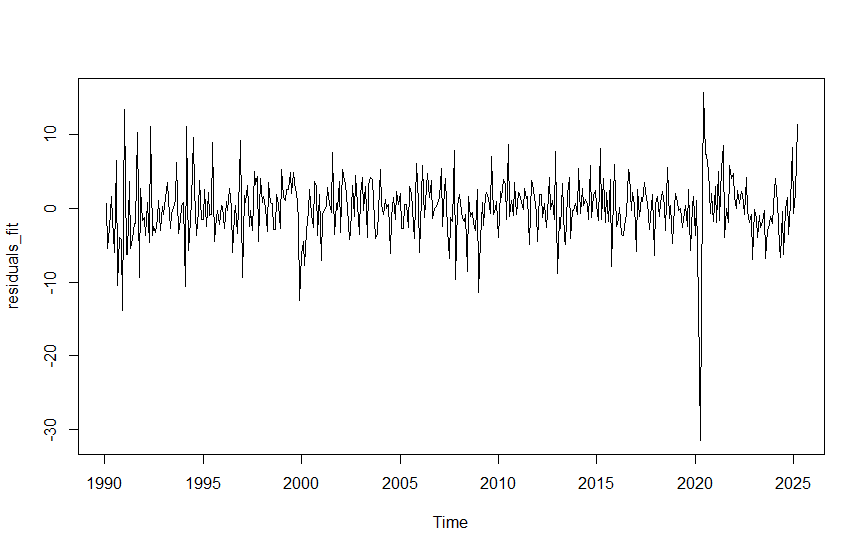
\includegraphics[width=0.5\linewidth]{plot residuals.png}
            \caption{Plot of residuals}
            \label{fig:plot_residuals}
        \end{figure}
        %
        \begin{table}[ht]
            \centering
            \begin{tabular}{l|cc}
                \textbf{df} & \(\chi^2\) & \textbf{p-value} \\
                \hline
                22 & 31.287 & 0.0904 \\
            \end{tabular}
            \caption{Ljung-Box test for lag 24 on residuals}
            \label{tab:ljung_box}
        \end{table}

        To conclude, we have picked the $\ARMA(1, 1)$ model for the series $(\nabla Y_t)$. It is valid because we have tested both the stationarity of $(\nabla Y_t)$ and the fact that the residual is a white noise.

        \item We have $(\nabla Y_t) \sim \ARMA(1, 1)$, thus $(Y_t) \sim \ARIMA(1, 1, 1)$ with the coefficients estimated in Table \ref{tab:arma11_coeffs}:
        %
        \[\nabla Y_t = 0.0310 + 0.4253 \nabla Y_{t - 1} - 0.8458 \varepsilon_{t - 1} + \varepsilon_t, \qquad (\varepsilon_t) \sim \WN(0, \sigma^2)\]
    \end{enumerate}

    \section{Prediction}

    \begin{enumerate}
        \item Let $\phi$ and $\theta$ the coefficients predicted by $\hat\phi=-0.4253$ and $\hat\theta=-0.8458$. We have $|\hat\phi|<1$ and $|\hat\theta|<1$, thus, the $\ARMA(1,1)$ model for $(\nabla Y_t)$ has the following canonical representation:
        %
        \[\nabla Y_t - \phi \nabla Y_{t-1} = \varepsilon_t - \theta\varepsilon_{t-1}\]

        Where $\varepsilon_t$ is the linear innovation of the model. Thus:
        %
        \begin{equation} \label{innov}
        \mathbb{E}[\varepsilon_{t+h}|\mathcal{F}_t]=0, \qquad \forall h > 0
        \end{equation}

        The canonical representation gives us:
        %
        \begin{equation} \label{nabla}
        \begin{cases}
            \nabla Y_{t+1}=\phi\nabla Y_t - \theta\varepsilon_t + \varepsilon_{t+1} \\
            \nabla Y_{t+2} = \phi(\phi\nabla Y_t -\theta\varepsilon_t) + (\phi - \theta)\varepsilon_{t+1} + \varepsilon_{t+2}
        \end{cases}
        \end{equation}

        Letting $\widehat{\nabla Y}_{t+1|t} = \mathbb{E}[\nabla Y_{t+1}|\mathcal{F}_t]$ and $\widehat{\nabla Y}_{t+2|t} = \mathbb{E}[\nabla Y_{t+2}|\mathcal{F}_t]$, \eqref{innov} gives us:

        \begin{equation} \label{nablahat}
        \begin{cases}
            \widehat{\nabla Y}_{t+1}=\phi\nabla Y_t - \theta\varepsilon_t \\
            \widehat{\nabla Y}_{t+2} = \phi(\phi\nabla Y_t -\theta\varepsilon_t)
        \end{cases}
        \end{equation}

        Then, subtracting \eqref{nablahat} from \eqref{nabla} gives:

        \begin{equation} \label{nablaerr}
        \begin{cases}
            \nabla Y_{t+1} - \widehat{\nabla Y}_{t+1} = \varepsilon_{t+1} \\
            \nabla Y_{t+2} - \widehat{\nabla Y}_{t+2} = (\phi -\theta)\varepsilon_{t+1} + \varepsilon_{t+2}
        \end{cases}
        \end{equation}

        The predictions are given by the following relations:
        %
        \begin{equation} \label{forecast}            
        \begin{cases}
            \widehat{Y}_{t+1|t}=\widehat{\nabla Y}_{t+1|t} + Y_t \\
            \widehat{Y}_{t+2|t}=\widehat{\nabla Y}_{t+2|t} + Y_{t+1}
        \end{cases}
        \end{equation}
        
        Given $\nabla Y_{t+1} = Y_{t+1}-Y_t$ and the first lines of \eqref{nablaerr} and \eqref{forecast}, we obtain the prediction error at $t+1$:
        %
        \[ e_1 = Y_{t+1}-\widehat{Y}_{t+1|t}=\nabla Y_{t+1} - \widehat{\nabla Y}_{t+1|t} = \varepsilon_{t+1} \]

        Then, $\nabla Y_{t+2} = Y_{t+2} - Y_{t+1}$ and the second lines of \eqref{nablaerr} and \eqref{forecast} gives us the prediction error at $t+2$:
        %
        \[ e_2 = Y_{t+2} - \widehat{Y}_{t+2|t} = \nabla Y_{t+2} - \widehat{\nabla Y}_{t+2|t} = (\phi -\theta)\varepsilon_{t+1} + \varepsilon_{t+2} \]

        Knowing that $(\varepsilon_t) \sim \WN(0, \sigma^2)$, the prediction error covariance matrix is given by:
        %
        \[\Sigma = \Var\begin{pmatrix} e_1 \\ e_2\end{pmatrix} = \sigma^2\begin{pmatrix}
            1 & 1 + \phi - \theta \\
            1 + \phi - \theta & 1 + (1 + \phi - \theta)^2
        \end{pmatrix} \]

        Assuming that $(\varepsilon_t) \iidsim \mathcal{N}(0, \sigma^2)$, we then have a confidence region of level $\alpha$ given by the following relations:
        %
        \begin{align*}
            1-\alpha&=\mathbb{P}\left(Y_{t+1}\in\left[\widehat{Y}_{t+1|t} - q_{1-\alpha}\hat\sigma, \widehat{Y}_{t+1|t} + q_{1-\alpha}\hat\sigma\right]\right) \\
            1-\alpha&=\mathbb{P}\left(Y_{t+2}\in\left[\widehat{Y}_{t+2|t} - q_{1-\alpha}\hat\sigma \sqrt{ 1 + (1 + \phi - \theta)^2}, \widehat{Y}_{t+2|t} + q_{1-\alpha}\hat\sigma \sqrt{ 1 + (1 + \phi - \theta)^2}\right]\right)
        \end{align*}

        \item To obtain this confidence region, we assumed:
        \begin{itemize}
            \item Our $\ARMA(1,1)$ model being well specified.
            \item $(\varepsilon_t) \iidsim \mathcal{N}(0, \sigma^2)$
            \item $\widehat{Y}_{t+1}$ and $\widehat{Y}_{t+2}$ being consistent
        \end{itemize}

        \item The 95\% confidence region is represented in Figure \ref{fig:confidence_region}. We have $\begin{pmatrix} \widehat{Y}_{t+1|t} \\ \widehat{Y}_{t+2|t}\end{pmatrix} = 
        \begin{pmatrix} 102.23 \\ 99.99\end{pmatrix}$.
        %
        \begin{figure}[h]
            \centering
            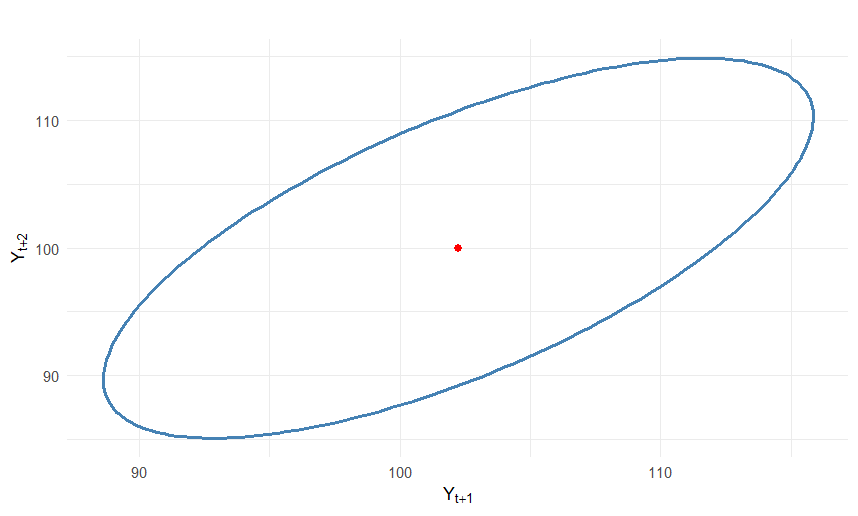
\includegraphics[width=0.9\linewidth]{plot region.png}
            \caption{Confidence region of $(Y_{t+1},Y_{t+2})$ for $\alpha=95\%$}
            \label{fig:confidence_region}
        \end{figure}

        \item Let $(X_t)$ and $(Y_t)$ two time series with $(Y_t)$ assumed to be stationary. We observe $Y_{t+1}$ before $X_{t+1}$. This helps us improve the prediction of $X_{t+1}$ if and only if $(Y_t)$ causes $(X_t)$ instantaneously in the Granger sense, that is:
        %
        \[\mathbb{E}[X_{t+1}|\mathcal{F}_t,Y_{t+1}] \neq \mathbb{E}[X_{t+1}|\mathcal{F}_t]\]

        This is the case when the prediction errors of $(X_t)$ and $(Y_t)$ are correlated. Such an hypothesis can be tested by building an autoregressive vector model (VAR) of the joint distribution of $(X_t)$ and $(Y_t)$ and implementing a Wald test on the least squares estimated coefficients of said VAR model.
        
    \end{enumerate}

    \section{Appendix: source code}

    \begin{lstlisting}[language=R]
    # --- Packages & imports ---

    library(tseries)
    library(readr)
    library(tsibble)
    library(lubridate)
    library(ggplot2)
    library(forecast)
    library(patchwork)
    library(dplyr)
    library(lmtest)
    library(zoo)
    
    # Processing data
    raw <- read_delim(
      "data.csv",
      delim = ";",
      col_names = FALSE,
      show_col_types = FALSE
    )
    raw_month <- raw[ grepl("^\\d{4}-\\d{2}$", raw$X1) , ]
    min_date <- ymd(paste0(tail(raw_month$X1, 1), "-01")) # 1990-01-01
    y <- ts(
      rev(as.numeric(raw_month$X2)),
      start = c(year(min_date), month(min_date)),
      frequency = 12
    )
    
    plot(y)
    
    # Testing stationarity
    adf.test(y)
    pp.test(y)
    kpss.test(y)
    
    # Testing stationarity on first-order differenced series
    y_diff <- diff(y)
    plot(y_diff)
    adf.test(y_diff)
    pp.test(y_diff)
    kpss.test(y_diff)
    
    # Plot autocorrelation and partial autocorrelation of the differenced series
    acf(zoo(coredata(y_diff)), plot = TRUE, main = 'ACF of the differenced series')
    pacf(zoo(coredata(y_diff)), plot = TRUE, main = 'PACF of the differenced series')
    
    # AIC and BIC minimization
    max_p <- 7
    max_q <- 13
    results <- data.frame(p = integer(), q = integer(), AIC = numeric(), BIC = numeric())
    for (p in 0:max_p) {
      for (q in 0:max_q) {
        cat("Fitting ARMA(", p, ",", q, ")...\n")
        try({
          model <- Arima(y_diff, order = c(p, 0, q), include.mean = TRUE)
          results <- rbind(results, data.frame(
            p = p,
            q = q,
            AIC = AIC(model),
            BIC = BIC(model)
          ))
        }, silent = TRUE)
      }
    }
    best_aic <- results[which.min(results$AIC), ]
    best_bic <- results[which.min(results$BIC), ]
    print("Best model according to AIC:")
    print(best_aic) # ---> ARMA(4, 4)
    print("Best model according to BIC:")
    print(best_bic) # ---> ARMA(1, 1)
    
    # Significance of the coefficients in ARMA(4, 4) and ARMA(1, 1)
    fit_aic <- Arima(y_diff, order = c(4, 0, 4))
    fit_aic
    coeftest(fit_aic)
    fit_bic <- Arima(y_diff, order = c(1, 0, 1))
    fit_bic
    coeftest(fit_bic)
    
    # Uncorrelation test on the residuals of ARMA(1, 1)
    residuals_fit <- residuals(fit_bic)
    plot(residuals_fit)
    Box.test(residuals_fit, lag = 24, type = "Ljung-Box", fitdf = 2)
    
    
    # Joint confidence region for Y(t+1) and Y(t+2)
    
    fc <- forecast(fit_bic, h = 2)
    f1 <- as.numeric(fc$mean[1])
    f2 <- as.numeric(fc$mean[2])
    
    sigma2 <- fit_bic$sigma2
    phi    <- as.numeric(fit_bic$model$phi)
    theta  <- as.numeric(fit_bic$model$theta)
    
    # Compute the first MA weight for the stationary ARMA(1,1) on y_diff
    psi1 <- phi + theta
    
    # Variances and covariance of the 1-step and 2-step forecast errors for ΔY
    var1  <- sigma2 * (1 + theta^2)        # Var(e_{t+1})
    var2  <- sigma2 * (1 + psi1^2)         # Var(e_{t+2})
    cov12 <- sigma2 * psi1                 # Cov(e_{t+1}, e_{t+2})
    
    Sigma_d <- matrix(c(var1, cov12,
                        cov12, var2),
                      nrow = 2, byrow = TRUE)
    
    # Convert forecasts of ΔY into forecasts of Y
    y_last <- as.numeric(tail(y, 1))       # last observed Y_t
    mu_y1  <- y_last + f1                  # E[Y_{t+1}]
    mu_y2  <- y_last + f1 + f2             # E[Y_{t+2}]
    center <- c(mu_y1, mu_y2)
    
    # Transformation matrix
    A <- matrix(c(1, 0,
                  1, 1),
                nrow = 2, byrow = TRUE)
    
    # Covariance matrix for the joint forecast error of (Y_{t+1}, Y_{t+2})
    Sigma_y <- A %*% Sigma_d %*% t(A)
    
    # Compute the points on the 95% confidence ellipse
    chisq_val <- qchisq(0.95, df = 2)
    eig <- eigen(Sigma_y)
    
    # Scale eigenvectors by sqrt(eigenvalues * khi2(0.95))
    transformation_matrix <- eig$vectors %*% diag(sqrt(eig$values * chisq_val))
    
    theta_seq <- seq(0, 2 * pi, length.out = 200)
    ellipse_coords <- t(sapply(theta_seq, function(t) {
      center + transformation_matrix %*% c(cos(t), sin(t))
    }))
    
    ellipse_df <- data.frame(
      Y_tp1 = ellipse_coords[, 1],
      Y_tp2 = ellipse_coords[, 2]
    )
    
    # Plot the 95% confidence ellipse
    ggplot(ellipse_df, aes(x = Y_tp1, y = Y_tp2)) +
      geom_path(color = "steelblue", size = 1) +
      geom_point(aes(x = center[1], y = center[2]), color = "red", size = 2) +
      labs(
        x = expression(Y[t + 1]),
        y = expression(Y[t + 2]),
        title = ""
      ) +
      theme_minimal()
    \end{lstlisting}
\end{document}